\documentclass[8pt]{beamer}
\usepackage[utf8]{inputenc}
\usepackage{xcolor}
\usepackage{colortbl}
\usepackage{epsfig}
% \usepackage{cancel}
\usepackage{ulem}
% \usepackage{threeparttable} % Joao Pela: 
\usepackage{amsmath}
\usepackage{hyperref}
\usepackage{siunitx}  % Allows easy x10^ for numbers
\usepackage{appendixnumberbeamer}

\usetheme{Madrid}

\author[J. Pela]{João Pela}
\title{QCD VBFMET samples MadGraph: New proposal}
\institute[ICL]{Imperial College London}
\date{2015-09-01}

% The log drawn in the upper right corner.
\logo{\includegraphics[height=0.115\paperheight]{img/Logo_CMSICL.png}}

\begin{document}
\setlength{\unitlength}{1mm}

% ###################################################
\begin{frame}
  \titlepage
\end{frame}

% ###################################################
\begin{frame}{Introduction}

\begin{block}{In the last presentation}
  
\begin{itemize}
  \item Presented first results from MadGraph \texttt{pp>jj}
  \begin{itemize}
    \item Pythia8 hadronization efficiency
    \item Variable migration studies: parton $\rightarrow$ gen jets
  \end{itemize}
  \item Questions were raised about Pythia8 vs MadGraph for parton level cuts
\end{itemize}

\end{block}

\begin{block}{Pythia vs MadGraph}

From conversations with Josh Bendavid:

\begin{itemize}
  \item Yes, both madgraph and pythia also allow the implementation of custom cuts in the hard process.
  \item MadGraph is more flexible for cuts in general out of the box.
  \item Madgraph also does allow to include extra jets at the ME level (QCD samples produced for SUSY have 2,3,4 jets at ME level). 
  \begin{itemize}
    \item Better since these can also be included in the phase space cuts (ie you can require that any pair of jets satisfy your requirements).
  \end{itemize}
  \item We could manage to generate 1 single inclusive sample, without having to break things down in pthat bins.
\end{itemize}

\end{block}

\begin{center}
  So it was decided to proceed with studies with \uline{pp to 2, 3 and 4 jets} sample production.
\end{center}


\end{frame}


% ###################################################
\begin{frame}{Implementation of new MadGraph cuts}

After first multi-jet results came out and after checking MadGraph forums and direct code inspections it became clear mmjj cut was applied to all possible jet combinations.

\begin{block}{Implementing MadGraph Cuts}

\begin{itemize}
  \item Had to learn Fortran77 and reverse engineer MadGraph cuts code.
  \item Implemented cuts to select events with at least one dijet with:
  \begin{itemize}
    \item dijet\_pt: min pT of at least one jet pair
    \item dijet\_eta: min delta era of at least one jet pair
    \item dijet\_mjj: min invariant mass of at least one jet pair
  \end{itemize}
  \item According to Chayanit A. this can be integrated in the official MadGraph gridpacks for official production.
\end{itemize}

\end{block}

\begin{block}{Problems found at IC}

For a few days I was getting MadGraph crashes in specially long jobs (+10k diagrams)

\begin{itemize}
  \item Turns out MadGraph stores sub-process files at /tmp/ while running.
  \item At IC in most machines /tmp/ has its own partition and is limited in space to 1 GB.
  \item Big jobs would run out of space and crash.
  \item A work around was found with Simon to redirect temporary storage in the jobs.
\end{itemize}
  
\end{block}

\end{frame}

% ###################################################
\begin{frame}{Checking Correct Implementation (Parton level)}

% \vspace{-30px}
\begin{center}
\tiny
This plots are for pp to 2, 3 and 4 jets.
\end{center}
\vspace{-10px}

\begin{block}{Parton distributions - Cuts $p_\perp>40$, $\eta<5.0$, $\Delta\eta>3.0$ and $m_{jj}>800$}
  
\begin{columns}
  
\column[t]{0.30\linewidth}  
  \centering
  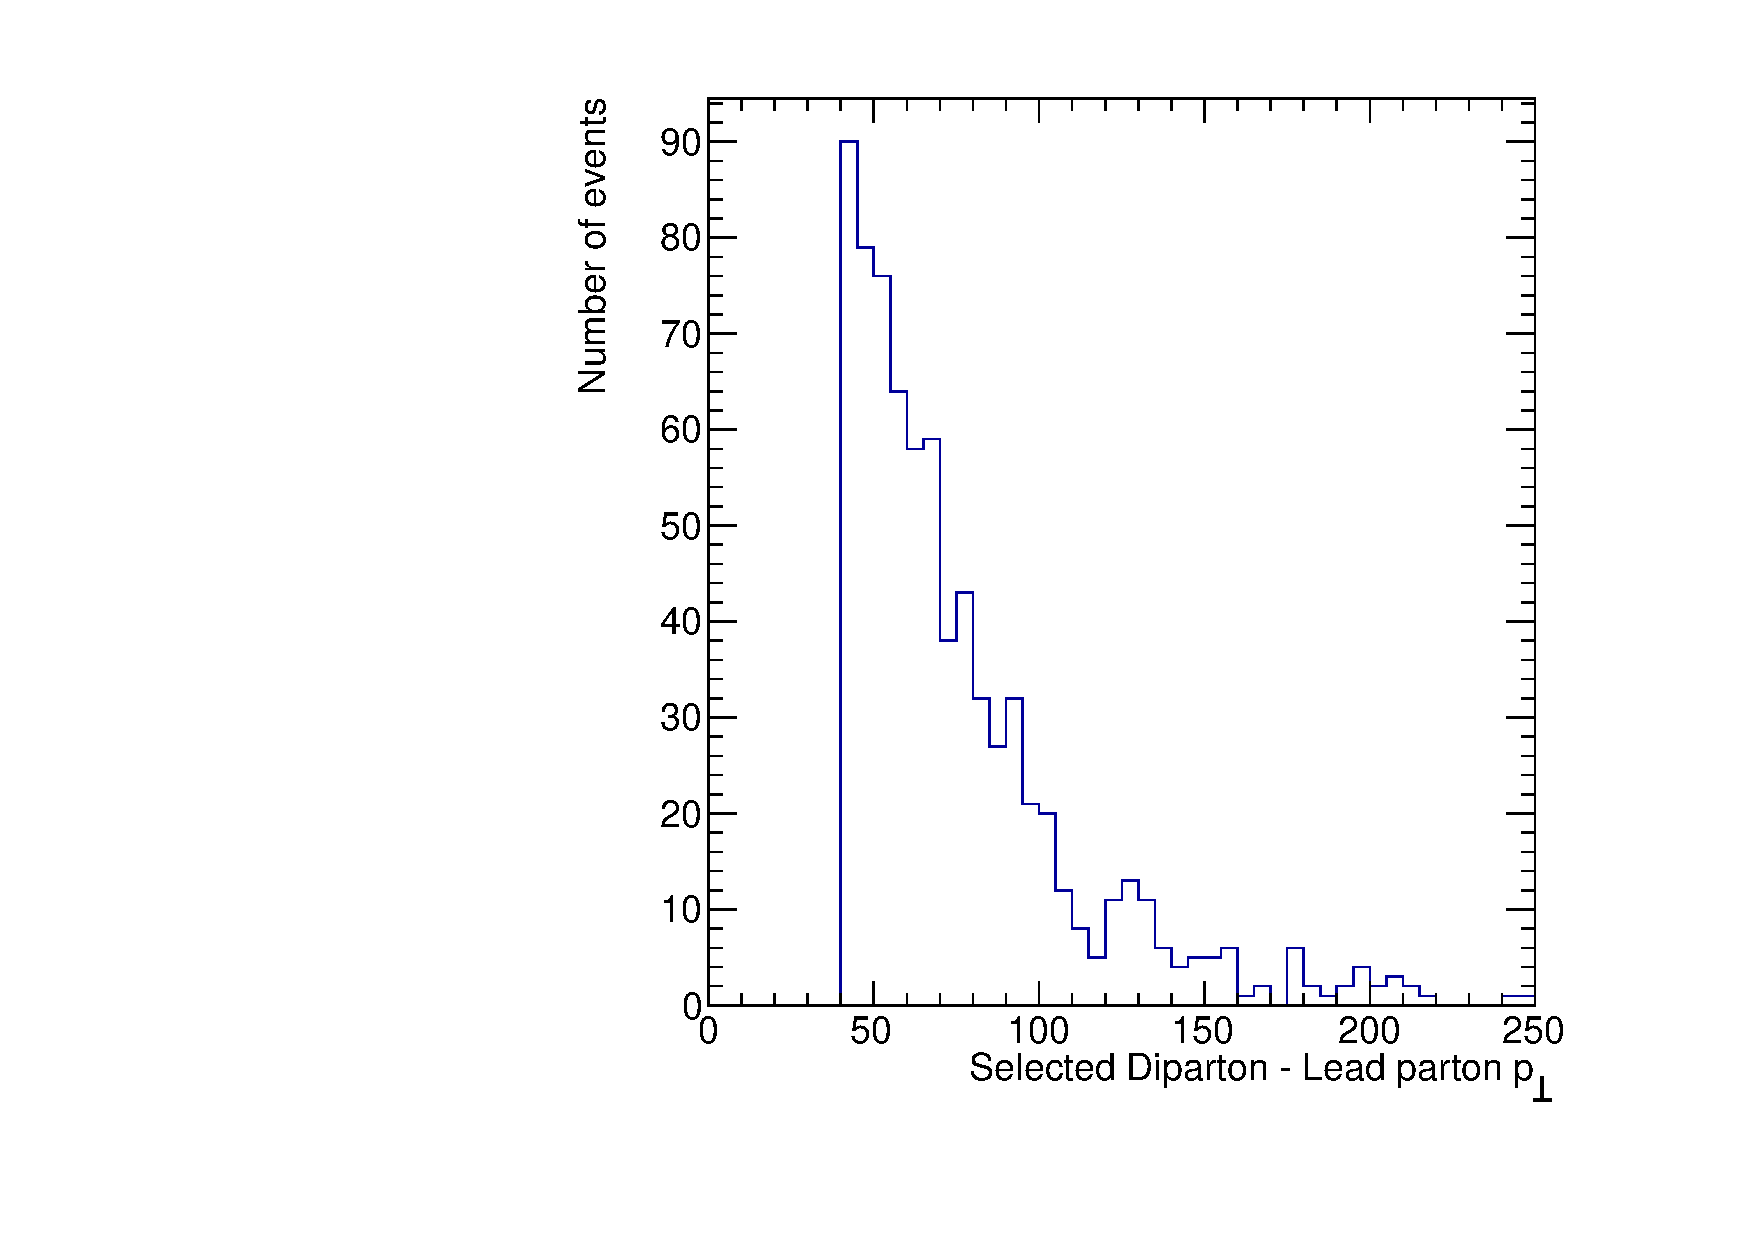
\includegraphics[width=0.8\linewidth]{img/SelDiParton_Parton1_Pt.pdf} \\
  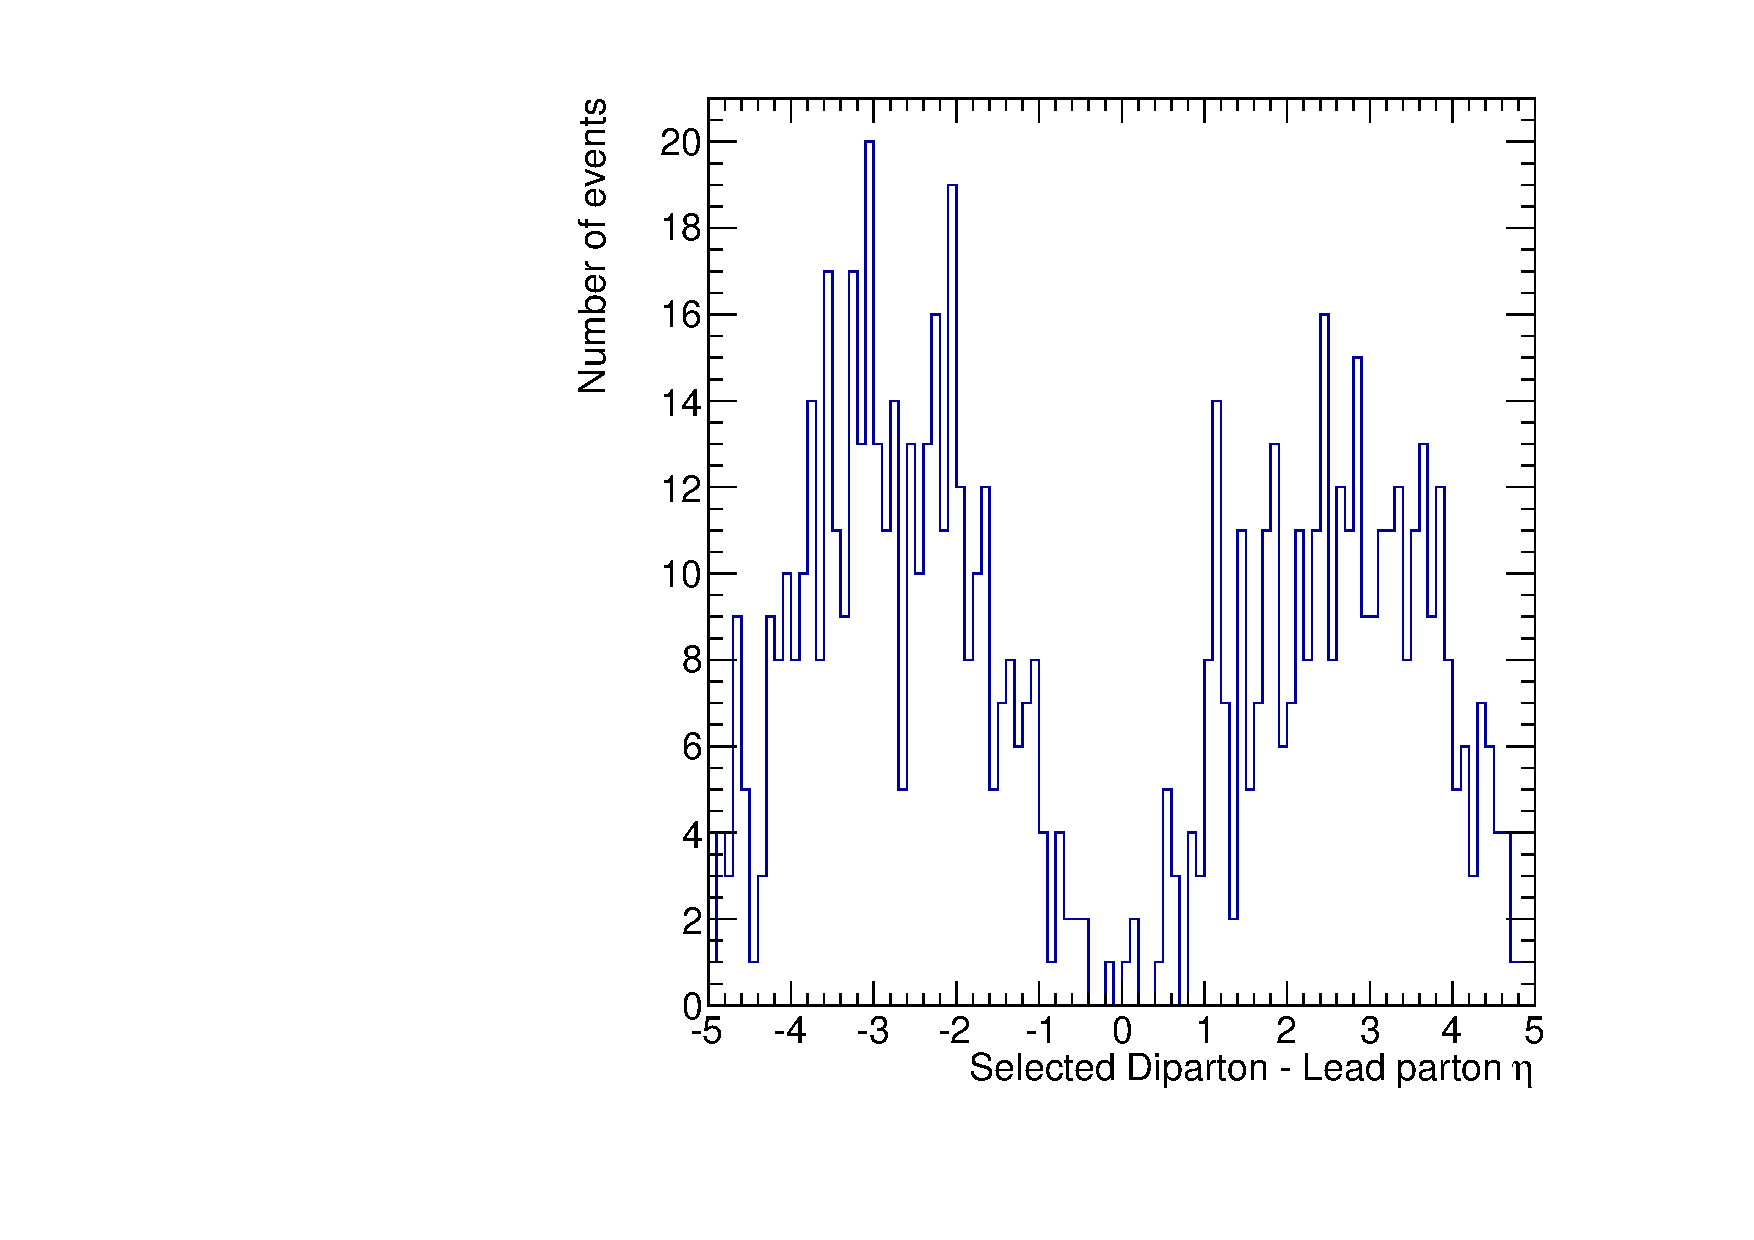
\includegraphics[width=0.8\linewidth]{img/SelDiParton_Parton1_Eta.pdf}
  
\column[t]{0.30\linewidth}
  \centering
  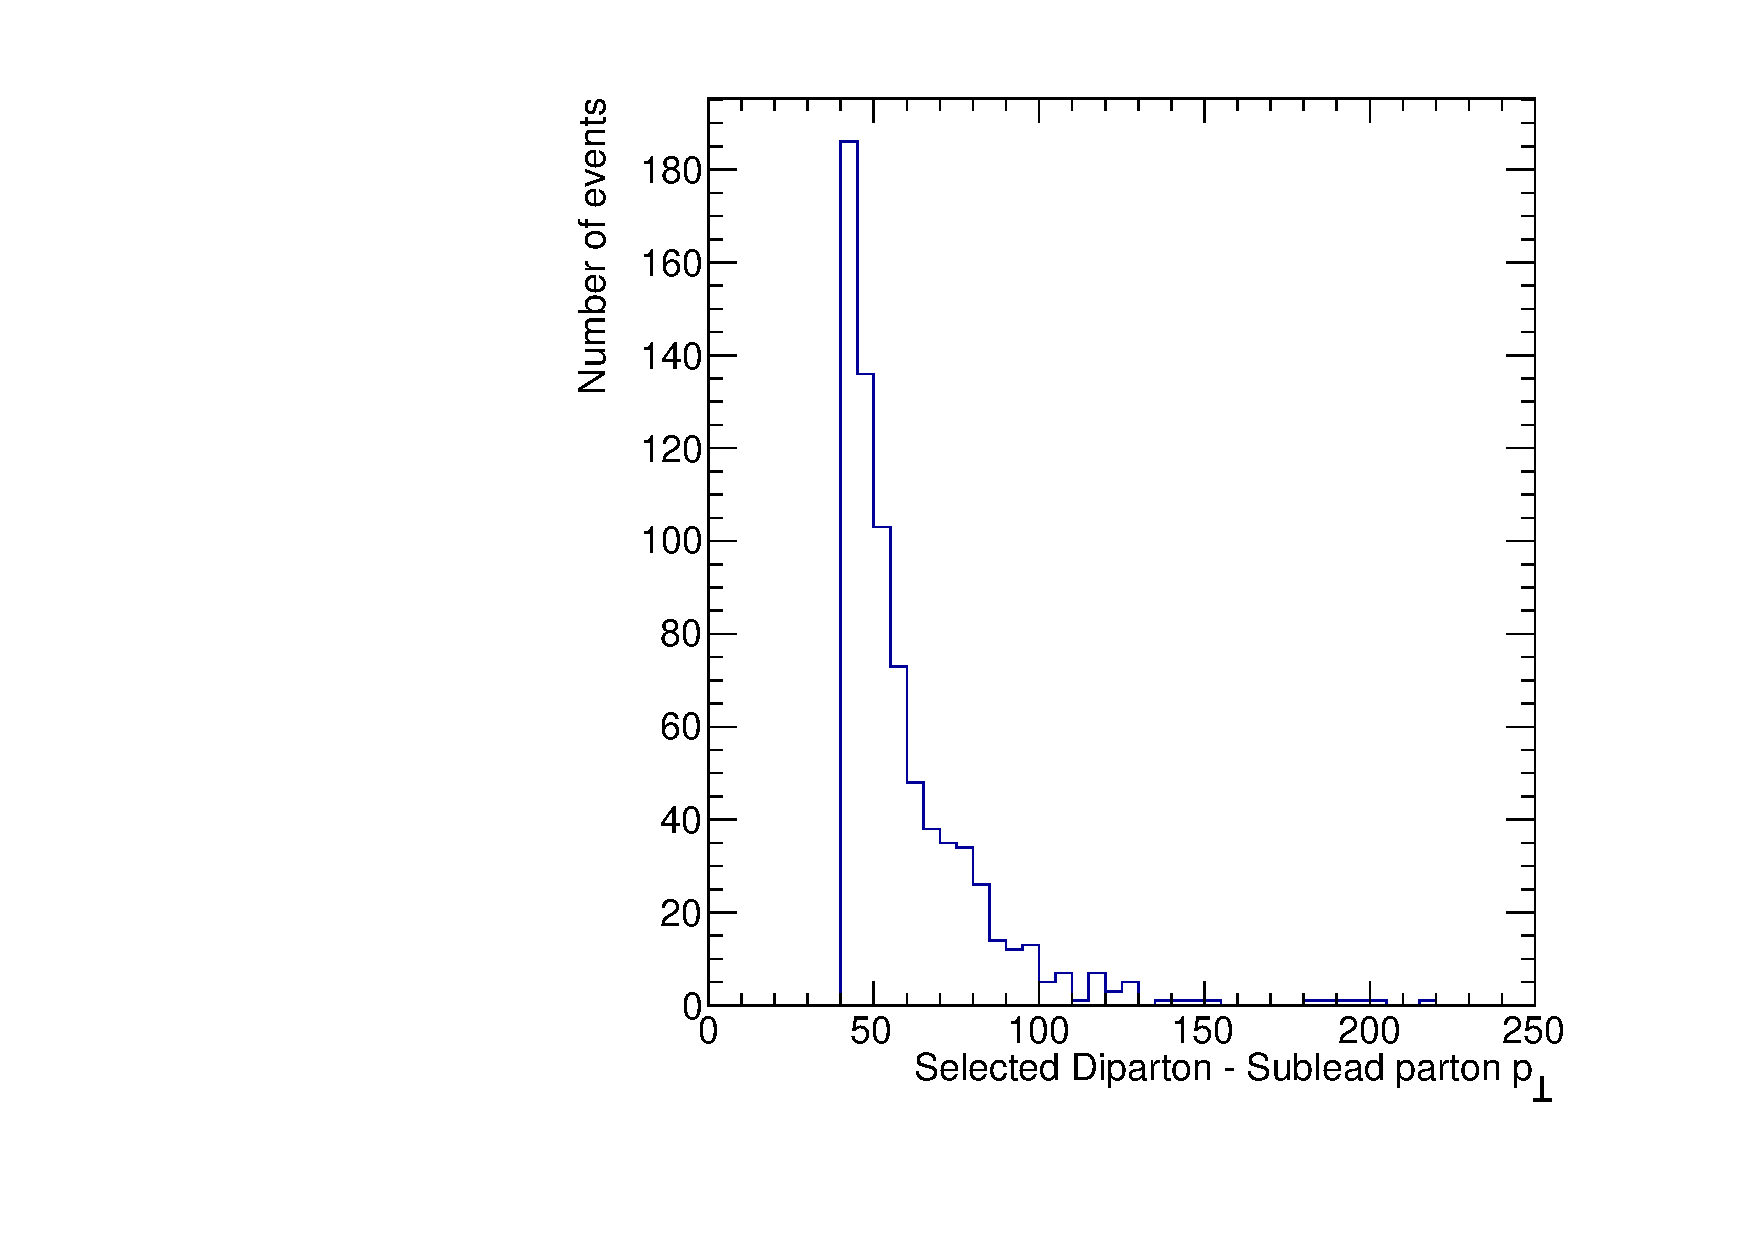
\includegraphics[width=0.8\linewidth]{img/SelDiParton_Parton2_Pt.pdf} \\
  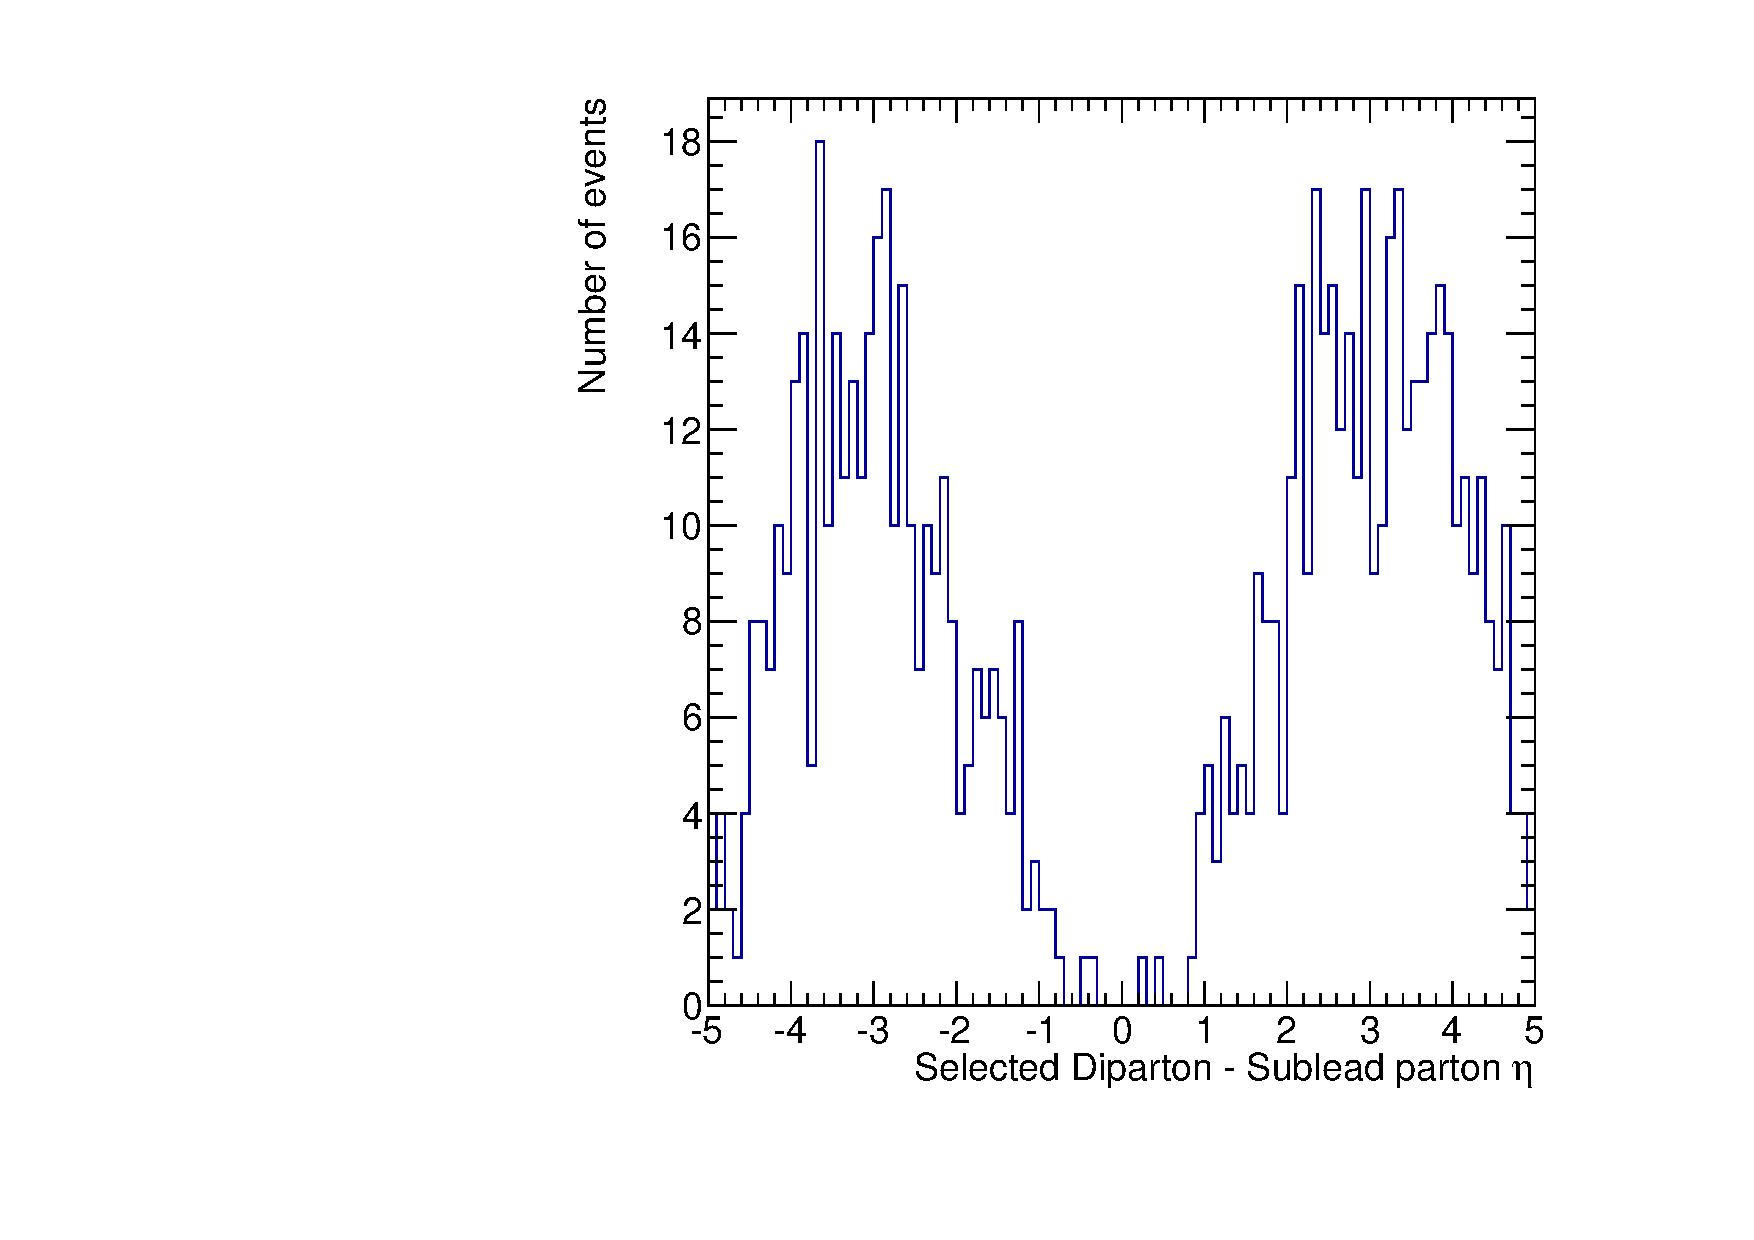
\includegraphics[width=0.8\linewidth]{img/SelDiParton_Parton2_Eta.pdf}

\column[t]{0.30\linewidth}
  \centering
  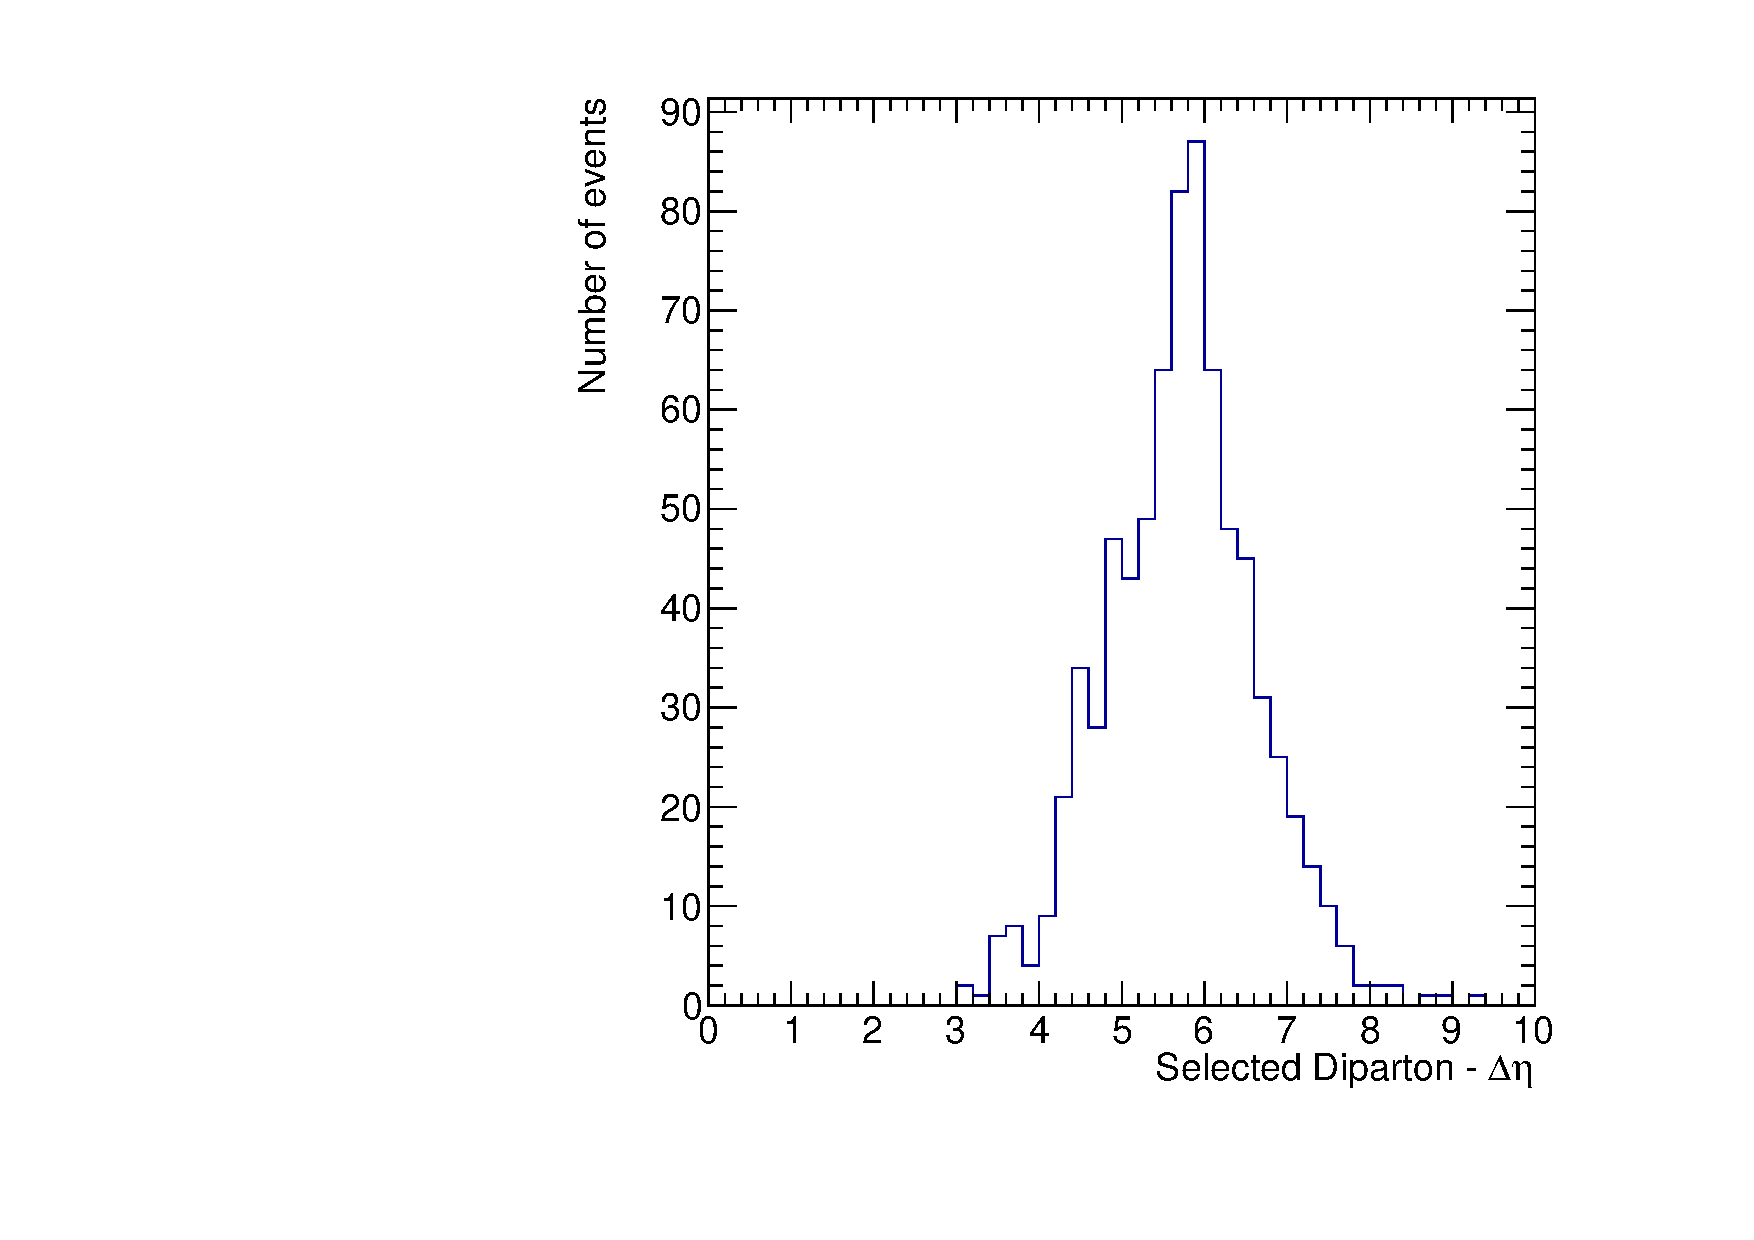
\includegraphics[width=0.8\linewidth]{img/SelDiParton_DEta.pdf} \\
  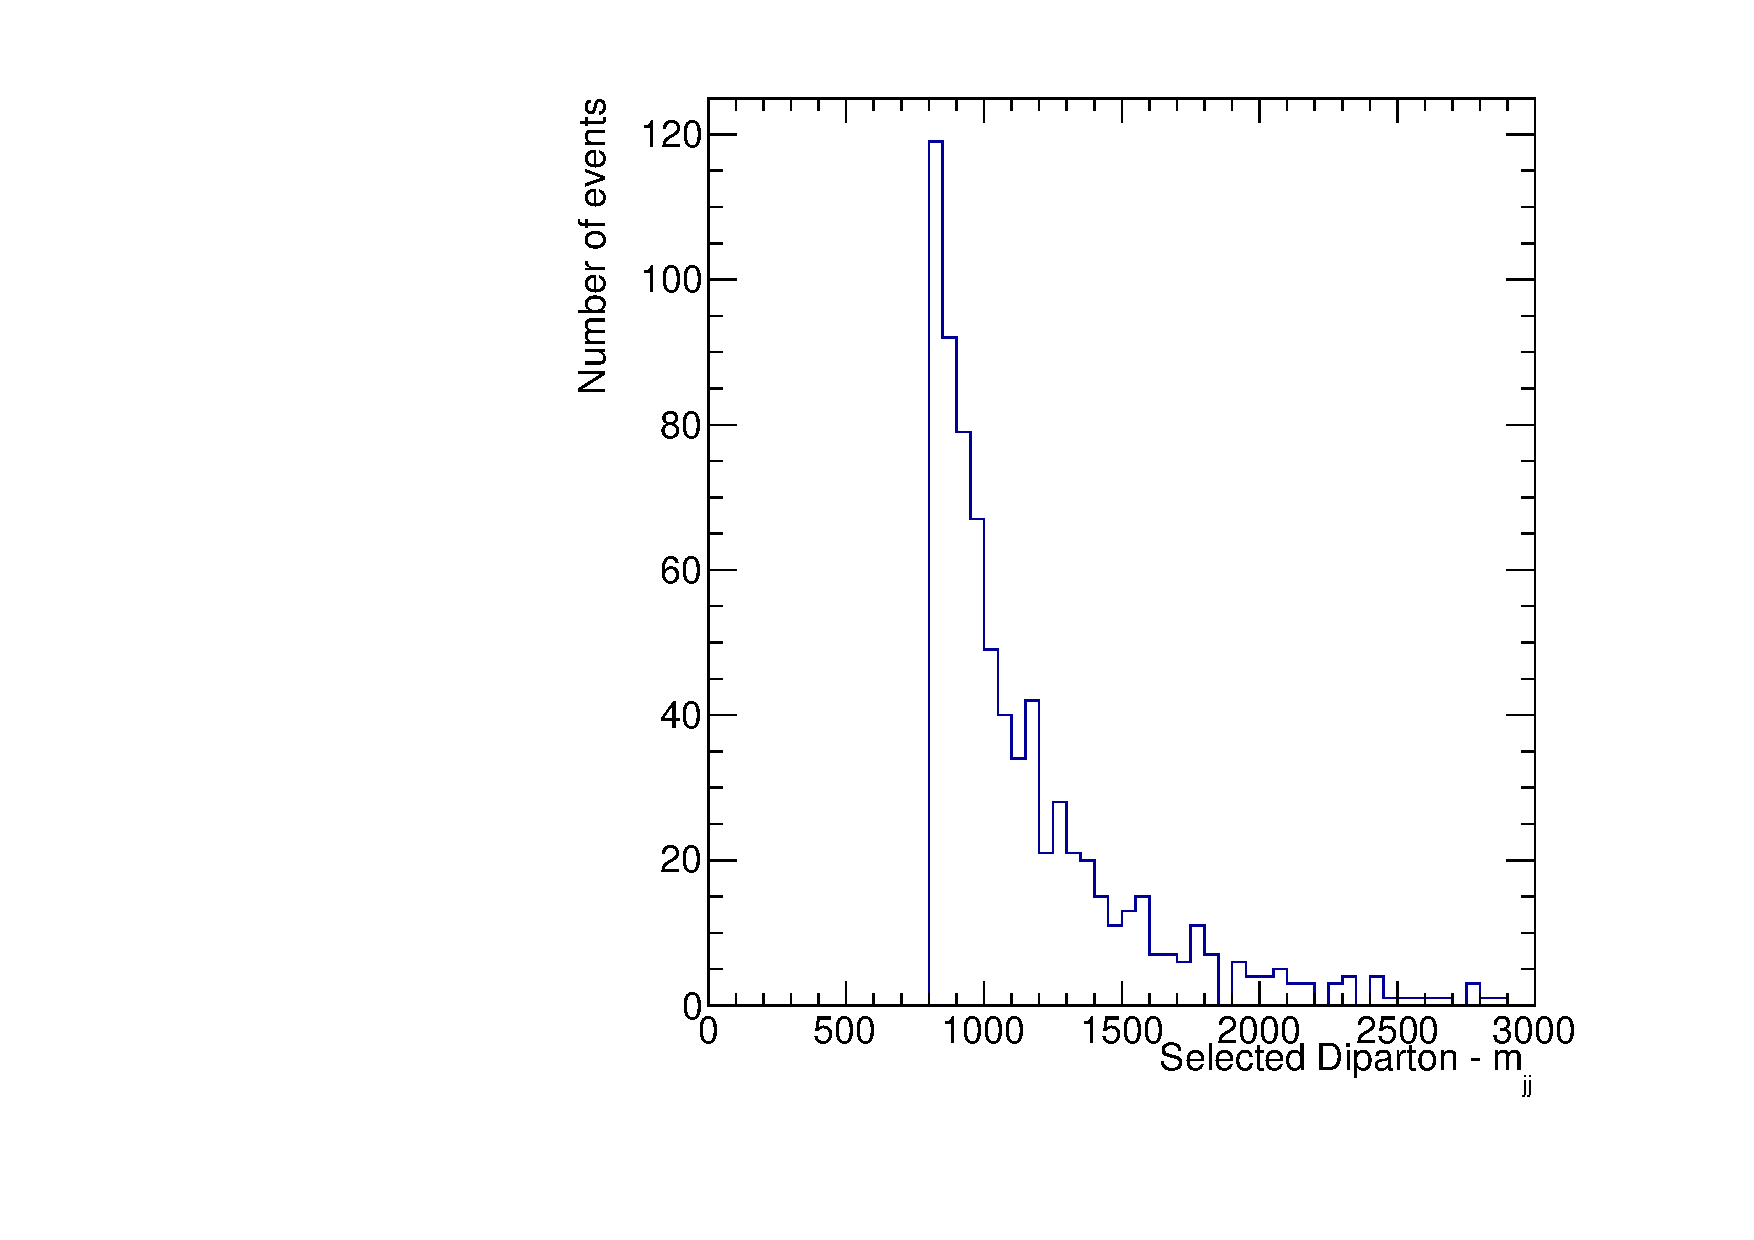
\includegraphics[width=0.8\linewidth]{img/SelDiParton_Mjj.pdf}

\end{columns}
  
\end{block}
  
\tiny
\begin{itemize}
  \item Cuts look like they are correctly implemented
  \item It can be seen here and also in my studies $\Delta\eta$ cut provides almost no reduction power below 4. We should not use this cut at parton level.
\end{itemize}
  
\end{frame}


% ###################################################
\begin{frame}{Obtained cross sections}

\begin{columns}
  
\column[t]{0.40\linewidth}


\begin{block}{$p_\perp>30$, $m_{jj}>800$}

\centering\tiny
\begin{tabular}{|l|c|}
\hline
Process          & Cross section [pb] \\
\hline
\hline                                               
\texttt{pp>jj}   & $\num{1.736e+06}\pm\num{4.477e+03}$ \\
\texttt{pp>jjj}  & $\num{3.977e+06}\pm\num{1.173e+04}$ \\
\texttt{pp>jjjj} & $\num{5.516e+06}\pm\num{1.248e+04}$ \\
\hline\hline
\texttt{pp>all}  & $\num{ 1.11e+07}\pm\num{1.799e+04}$ \\ 
\hline
\end{tabular}
  
\end{block}

\begin{block}{$p_\perp>30$, $\Delta\eta>2.5$, $m_{jj}>800$}

\centering\tiny 
\begin{tabular}{|l|c|}
\hline
Process          & Cross section [pb] \\
\hline
\hline                                               
\texttt{pp>jj}   & $\num{1.797e+06}\pm\num{4.594e+03}$ \\
\texttt{pp>jjj}  & $\num{3.804e+06}\pm\num{9.742e+03}$ \\
\texttt{pp>jjjj} & $\num{5.568e+06}\pm\num{1.083e+04}$ \\
\hline\hline
\texttt{pp>all}  & $\num{1.078e+07}\pm\num{1.946e+04}$ \\ 
\hline
\end{tabular}

\end{block}


\begin{block}{$p_\perp>40$, $\Delta\eta>3.0$, $m_{jj}>800$}
  
\centering\tiny
\begin{tabular}{|l|c|}
\hline
Process          & Cross section [pb] \\
\hline
\hline                                               
\texttt{pp>jj}   & $\num{8.621e+05}\pm\num{2.605e+03}$ \\
\texttt{pp>jjj}  & $\num{2.081e+06}\pm\num{4.714e+03}$ \\
\texttt{pp>jjjj} & $\num{3.186e+06}\pm\num{5.790e+03}$ \\
\hline\hline
\texttt{pp>all}  & $\num{5.7616e+06}\pm\num{1.2e+04}$ \\ 
\hline
\end{tabular}

\end{block}

\column[t]{0.50\linewidth}

\begin{block}{Conclusions}

\begin{itemize}
  \item $\Delta\eta$ cut only provides an event reduction of $\sim 5\%$
  \item With the least restrictive working point we can produce an 10 $fb^{-1}$ equivalent sample with $\sim 10^{11}$ parton level events.
  \item Compared with the Pythia8 study that implied full generation of $\num{2e12}$ events we have a factor 20 reduction.
  \item Hardest presented set cuts buys a further factor of 2 at the cost of less physics usability, but still under offline signal region cuts.
  \item Only caveat here is the size of such sample even at only parton level would be 20-30 TB (I think this is acceptable) 
  \item I will proceed presenting results for the least restrictive working point, but I have all number/plots for all working points
\end{itemize}

\end{block}

\end{columns}

\end{frame}

% ###################################################
\begin{frame}{Pythia8 Hadronization}

Next step is to proceed with Pythia8 Hadronization and matching.

\begin{block}{}
  
\resizebox{\linewidth}{!}{
\begin{tabular}{|l|c|c|c|c|c|c|}
\hline
                 &      & \multicolumn{3}{c|}{Events}    & \multicolumn{2}{c|}{Cross section [pb]}                                   \\
\hline
Process          &  \#  & Tried & Passed & Accepted [\%] & Pre-match                           & Post-match                          \\
\hline
\hline
\texttt{pp>jj}   &      & 10000 & 2197   & $22.0\pm0.4$  & $\num{1.736e+06}\pm\num{4.478e+03}$ & $\num{3.815e+05}\pm\num{7.256e+03}$ \\
\texttt{pp>jjj}  &      & 10000 & 696    & $ 7.0\pm0.3$  & $\num{3.977e+06}\pm\num{1.173e+04}$ & $\num{2.768e+05}\pm\num{1.015e+04}$ \\
\texttt{pp>jjjj} &      & 10000 & 581    & $ 5.8\pm0.2$  & $\num{5.517e+06}\pm\num{1.248e+04}$ & $\num{3.205e+05}\pm\num{1.293e+04}$ \\
\hline
\hline
\texttt{pp>all}  & jj   & 1454  & 312    & $21.5\pm1.1$  & $\num{1.617e+06}\pm\num{2.620e+03}$ & $\num{3.469e+05}\pm\num{1.741e+04}$ \\
\texttt{pp>all}  & jjj  & 3603  & 251    & $ 7.0\pm0.4$  & $\num{3.946e+06}\pm\num{6.394e+03}$ & $\num{2.749e+05}\pm\num{1.674e+04}$ \\
\texttt{pp>all}  & jjjj & 4943  & 337    & $ 6.8\pm0.4$  & $\num{5.538e+06}\pm\num{8.973e+03}$ & $\num{3.775e+05}\pm\num{1.986e+04}$ \\
\hline
\texttt{pp>all}  & all  & 10000 & 900    & $ 9.0\pm0.3$  & $\num{1.110e+07}\pm\num{1.132e+04}$ & $\num{9.993e+05}\pm\num{3.127e+04}$ \\
\hline
\end{tabular}
}

\end{block}

\end{frame}

% ###################################################
\begin{frame}{Matching Dipartons to Generator Dijets}

\begin{block}{Parton distributions}
  
\begin{columns}
  
\column[t]{0.30\linewidth}  
  \centering
  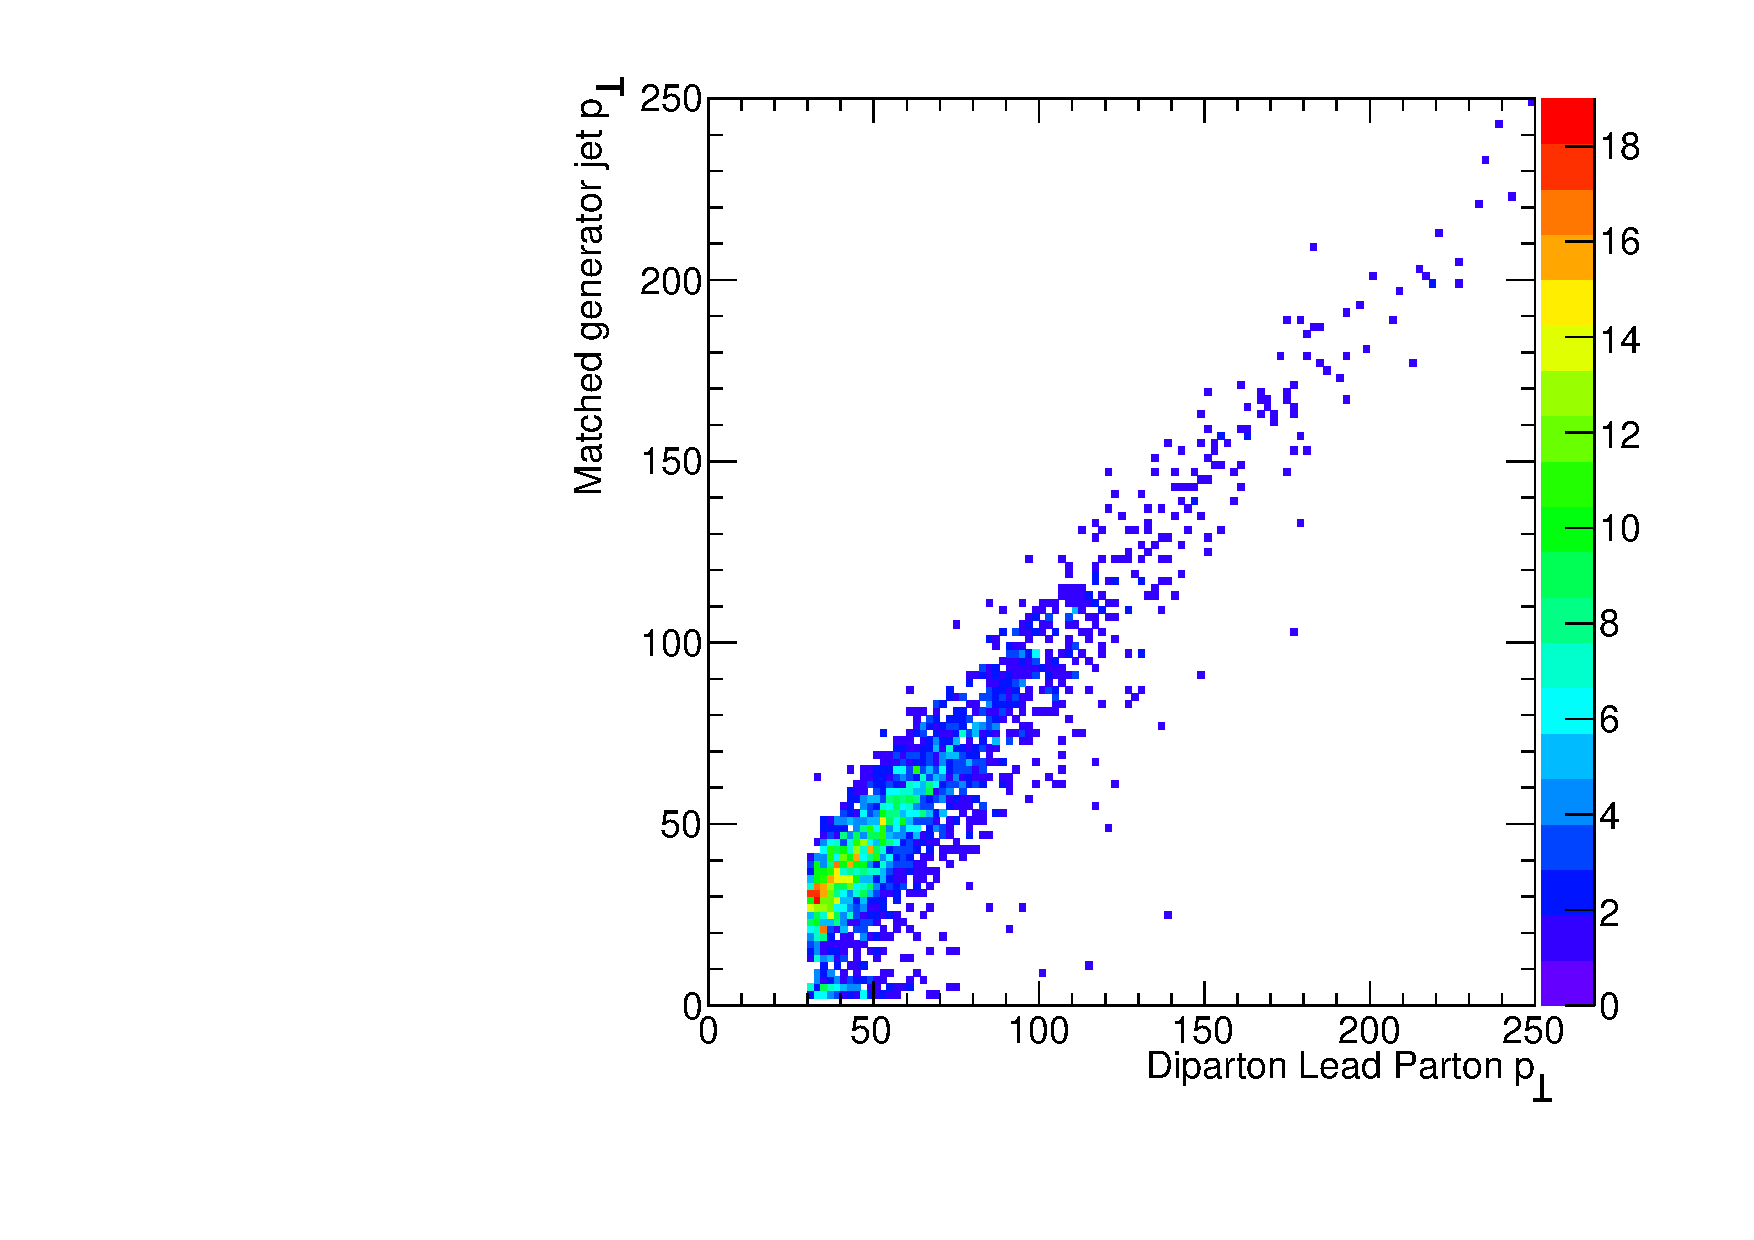
\includegraphics[width=0.8\linewidth]{img/SelDiParton_MatchedGenJet_Parton1_Pt.pdf} \\
  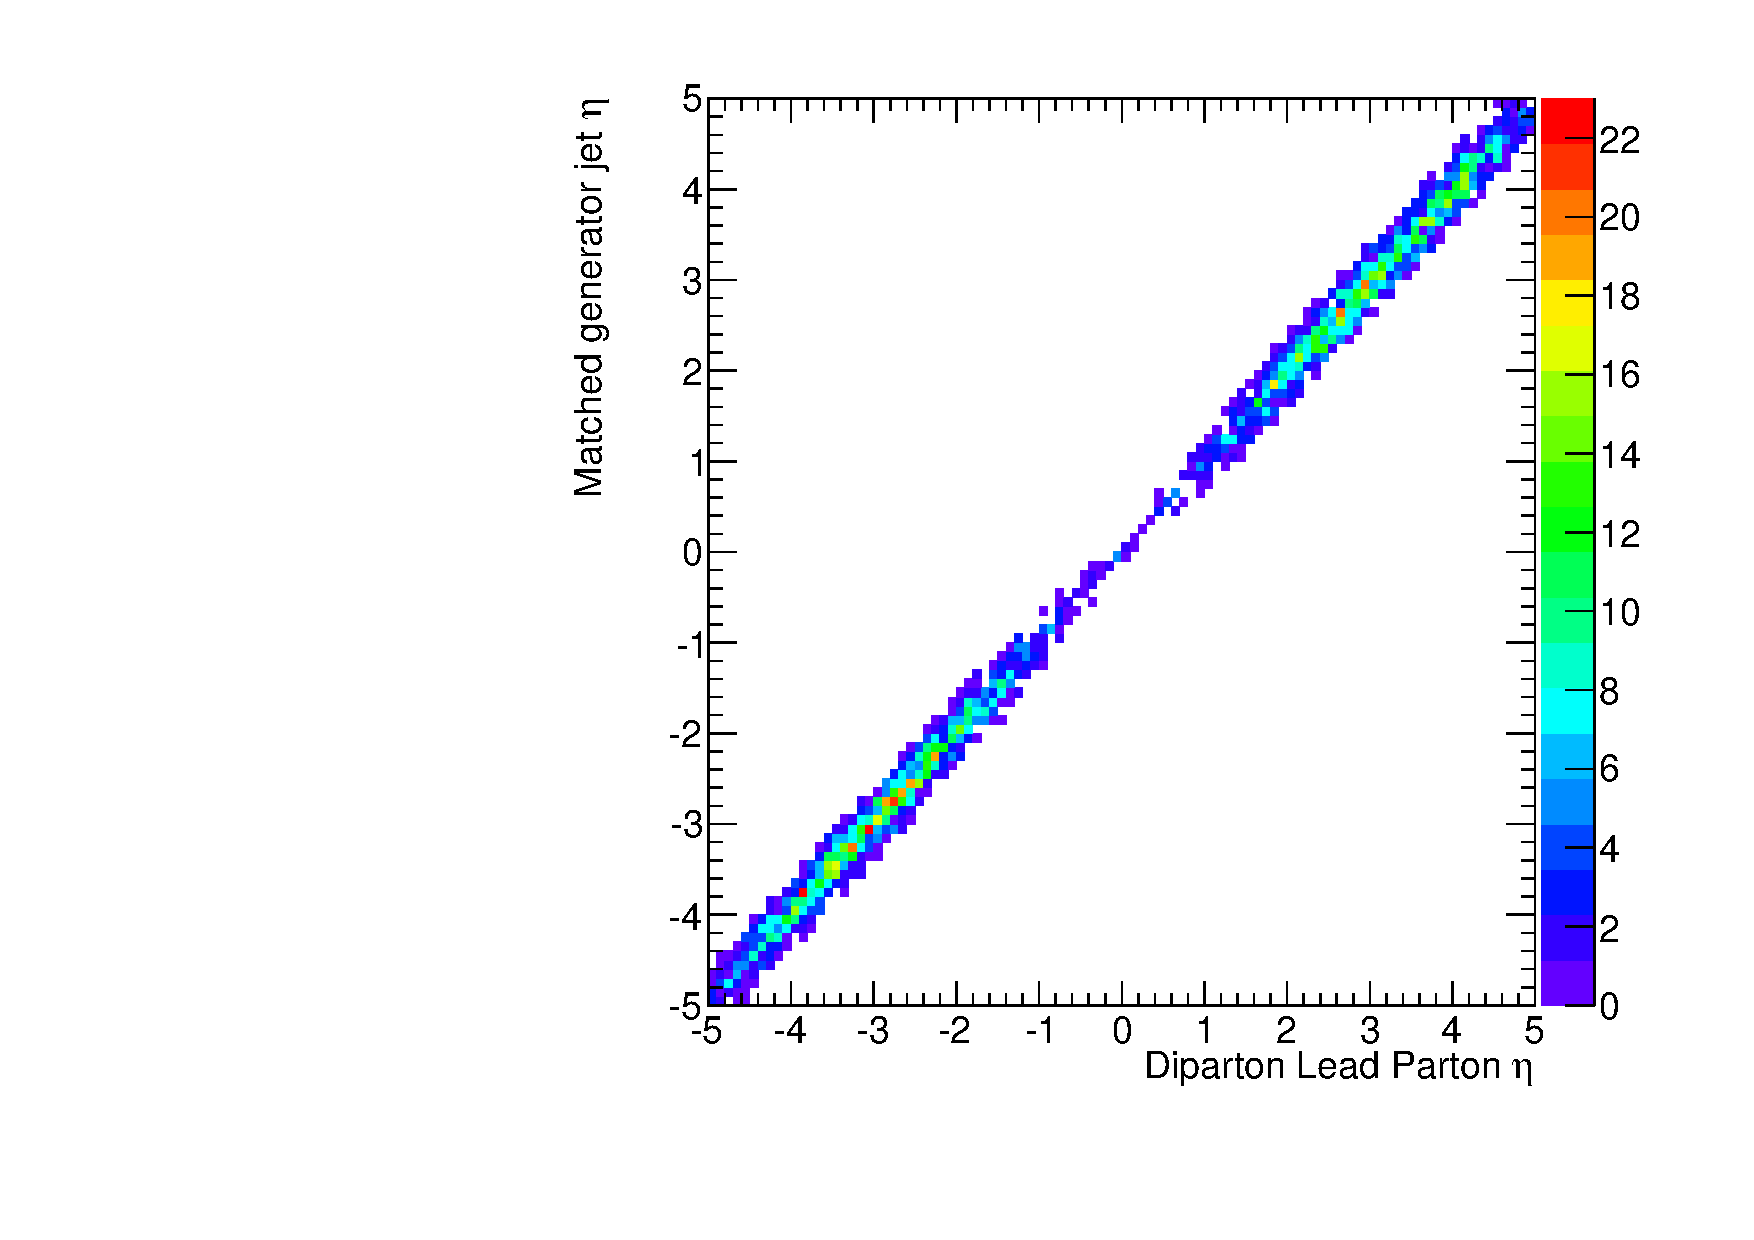
\includegraphics[width=0.8\linewidth]{img/SelDiParton_MatchedGenJet_Parton1_Eta.pdf}
  
\column[t]{0.30\linewidth}
  \centering
  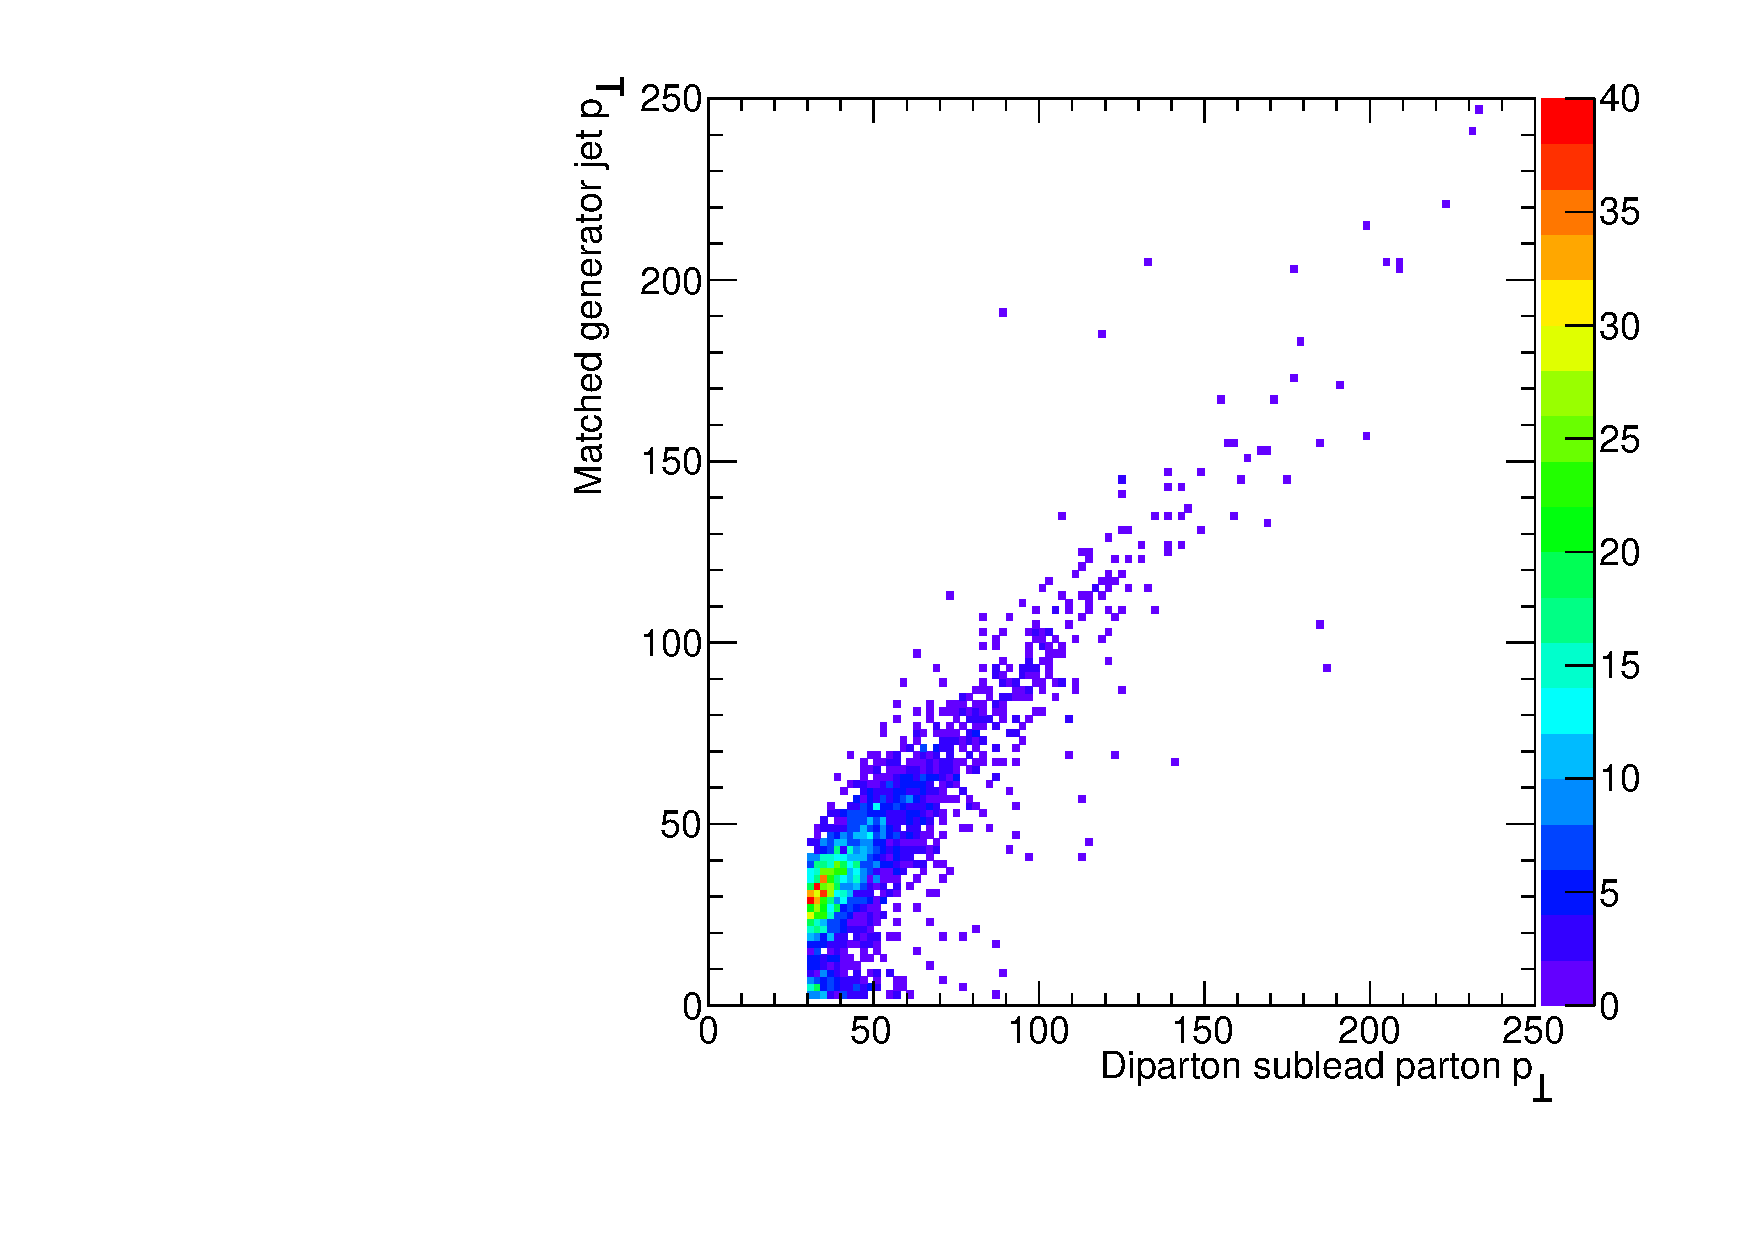
\includegraphics[width=0.8\linewidth]{img/SelDiParton_MatchedGenJet_Parton2_Pt.pdf} \\
  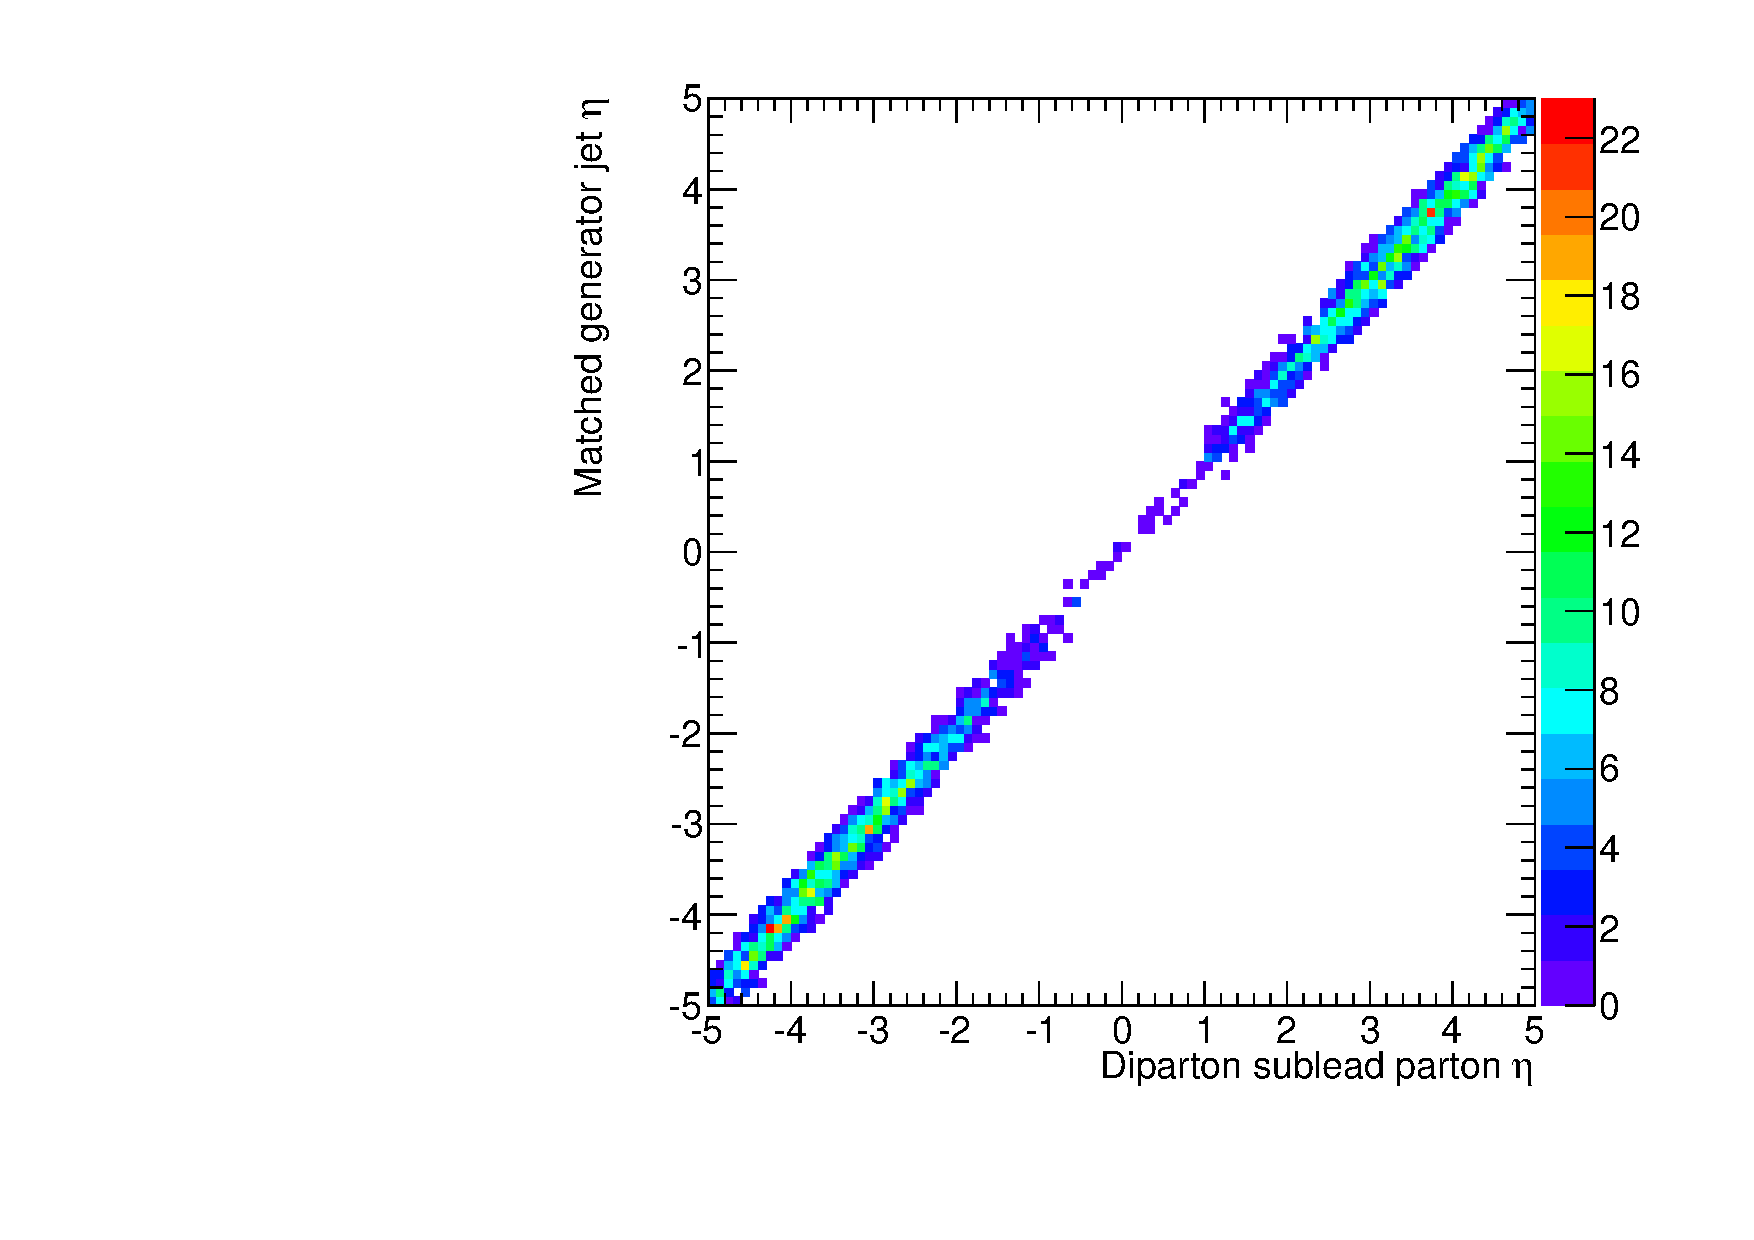
\includegraphics[width=0.8\linewidth]{img/SelDiParton_MatchedGenJet_Parton2_Eta.pdf}

\column[t]{0.30\linewidth}
  \centering
  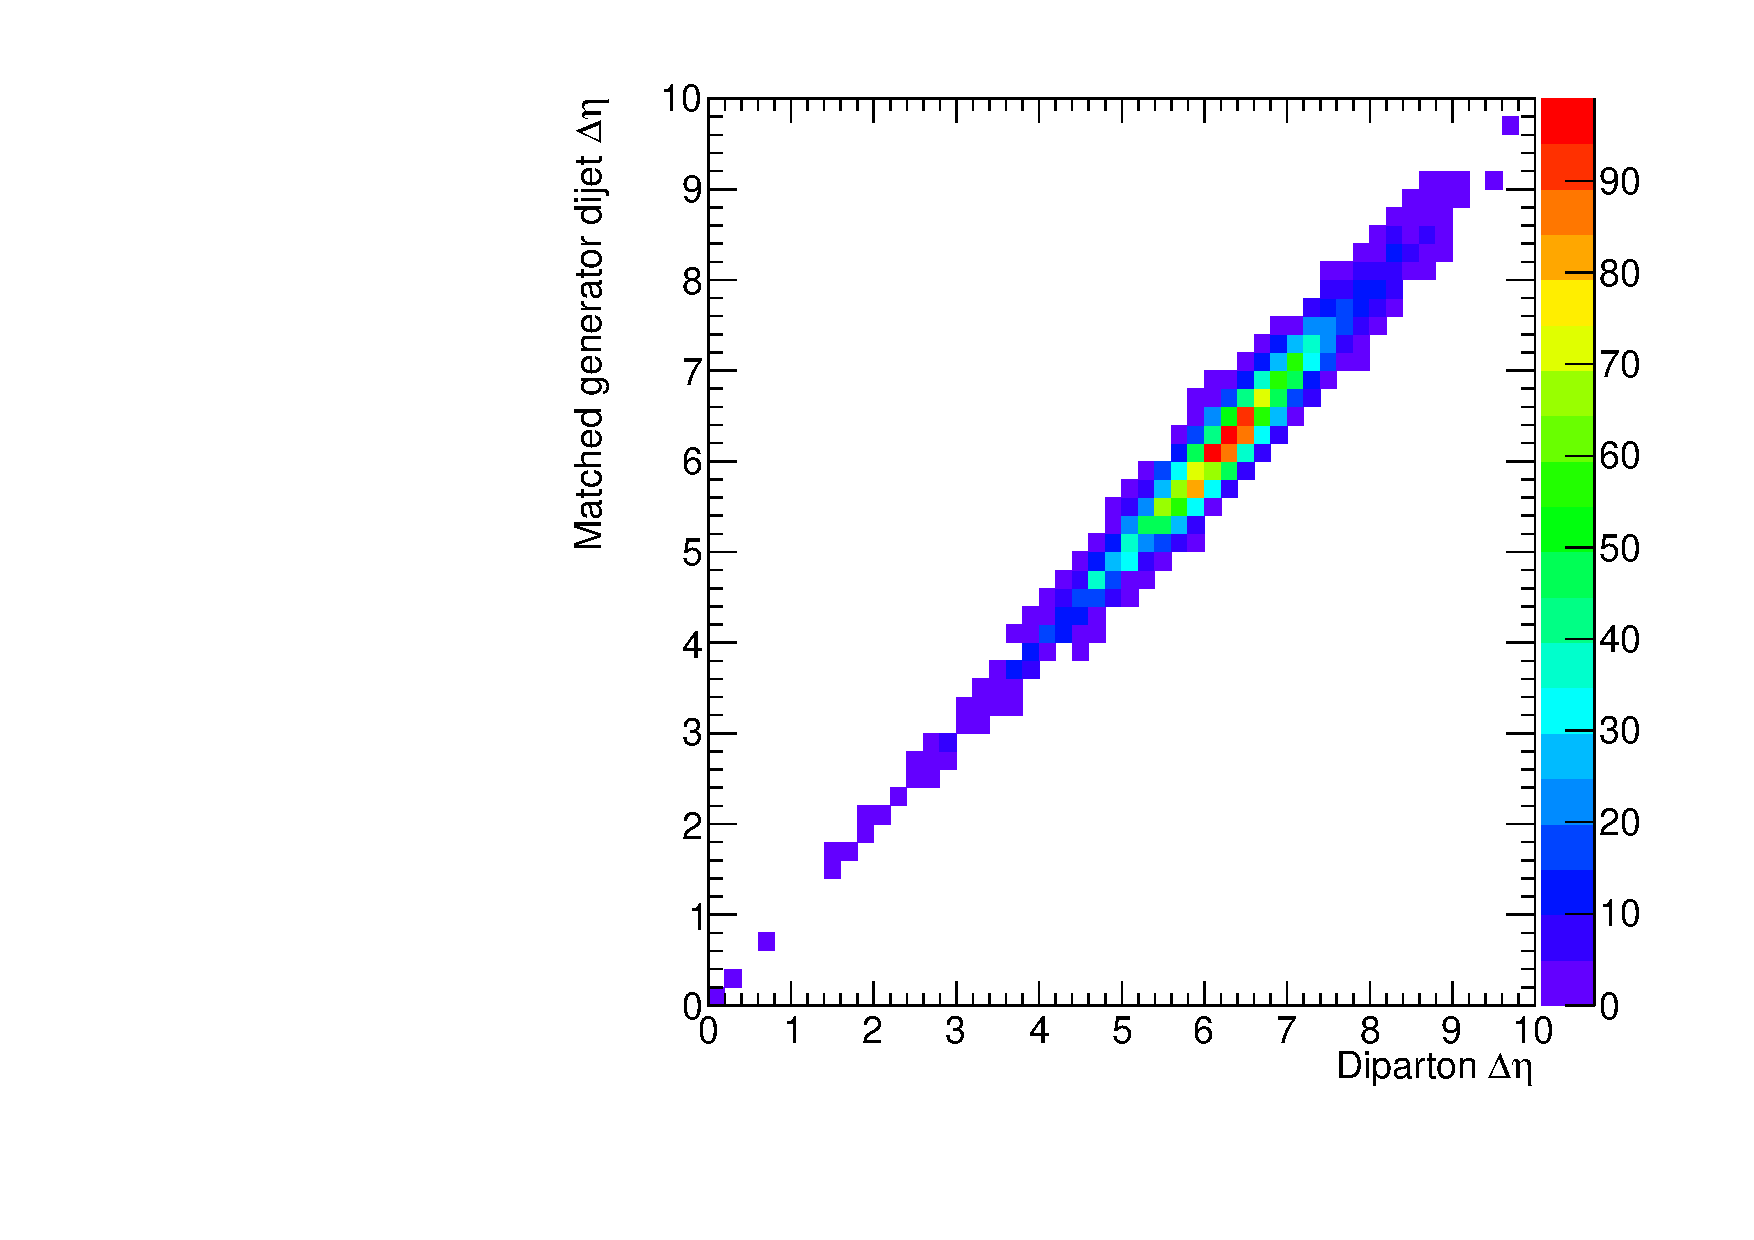
\includegraphics[width=0.8\linewidth]{img/SelDiParton_MatchedGenJet_DEta.pdf} \\
  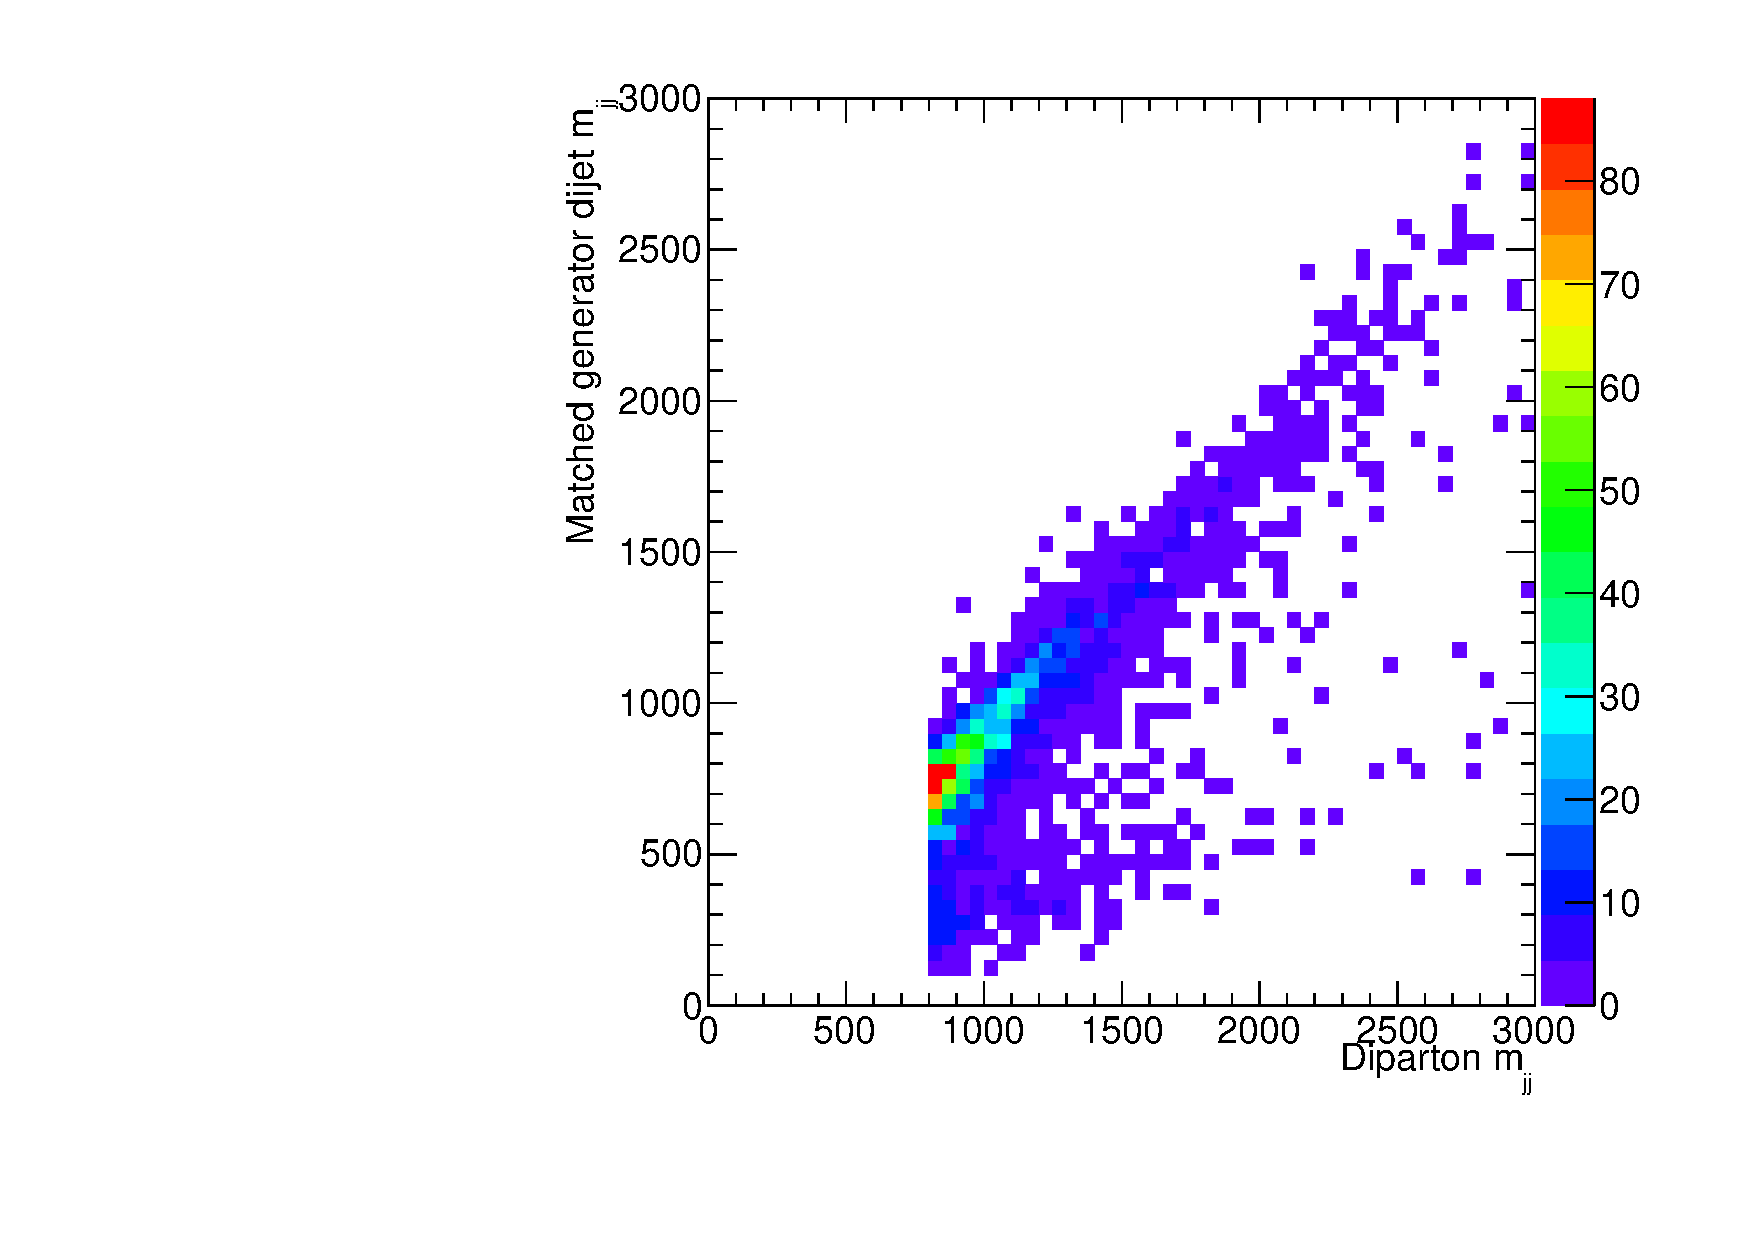
\includegraphics[width=0.8\linewidth]{img/SelDiParton_MatchedGenJet_Mjj.pdf}

\end{columns}
  
\end{block}

\begin{itemize}
  \item At the parton  $p_\perp$ cut line the upper tail of finishes around 50 GeV 
  \item At the diparton $m_{jj}$ cut line the upper tail of finishes around 1000 GeV    
  \item Good correlation in $\eta$ variables, but no migration problems since there is no cut at parton level
\end{itemize}


\end{frame}

% ###################################################
\begin{frame}{Filter efficiency}

Testing several generator filter configurations.

\begin{block}{Efficiencies and Expected events}
\centering

\resizebox{0.8\linewidth}{!}{
\begin{tabular}{|c|c|c|c|c||c|c|c|}
\hline
\multicolumn{5}{|c||}{Generator Cuts} & \multicolumn{2}{c|}{Results} \\
\hline
$p_\perp$ & $\eta$ & $\Delta\eta$ & $\Delta\phi$ & $m_{jj}$ & Filter Efficiency                   & Events for 10 $fb^-1$ \\
\hline
\hline
50        & 4.8    & 3.5          & -            & 1000     & $\num{8.248e-02}\pm\num{4.534e-03}$ & $\num{8.242e+08}\pm\num{4.530e+07}$ \\
\hline\hline
40        & 4.8    & 3.5          & 1.5          & 1000     & $\num{1.470e-02}\pm\num{1.914e-03}$ & $\num{1.469e+08}\pm\num{1.913e+07}$ \\
45        & 4.8    & 3.5          & 1.5          & 1000     & $\num{1.121e-02}\pm\num{1.672e-03}$ & $\num{1.121e+08}\pm\num{1.670e+07}$ \\
50        & 4.8    & 3.5          & 1.5          & 1000     & $\num{7.725e-03}\pm\num{1.387e-03}$ & $\num{7.719e+07}\pm\num{1.386e+07}$ \\
\hline\hline
50        & 4.8    & 3.5          & 1.5          & 800      & $\num{1.196e-02}\pm\num{1.726e-03}$ & $\num{1.195e+08}\pm\num{1.725e+07}$ \\
50        & 4.8    & 3.5          & 1.5          & 900      & $\num{9.718e-03}\pm\num{1.556e-03}$ & $\num{9.712e+07}\pm\num{1.555e+07}$ \\
\hline\hline
50        & 4.8    & 3.5          & 1.75         & 1000     & $\num{9.469e-03}\pm\num{1.536e-03}$ & $\num{9.463e+07}\pm\num{1.535e+07}$ \\
50        & 4.8    & 3.5          & 2.0          & 1000     & $\num{1.196e-02}\pm\num{1.726e-03}$ & $\num{1.195e+08}\pm\num{1.725e+07}$ \\
50        & 4.8    & 3.5          & 2.25         & 1000     & $\num{1.495e-02}\pm\num{1.930e-03}$ & $\num{1.494e+08}\pm\num{1.929e+07}$ \\
50        & 4.8    & 3.5          & 2.5          & 1000     & $\num{1.844e-02}\pm\num{2.144e-03}$ & $\num{1.843e+08}\pm\num{2.142e+07}$ \\
50        & 4.8    & 3.5          & 2.75         & 1000     & $\num{2.018e-02}\pm\num{2.243e-03}$ & $\num{2.017e+08}\pm\num{2.241e+07}$ \\
\hline\hline
50        & 4.8    & 3.0          & 1.5          & 1000     & $\num{7.725e-03}\pm\num{1.387e-03}$ & $\num{7.719e+07}\pm\num{1.386e+07}$ \\
50        & 4.8    & 3.0          & 2.0          & 1000     & $\num{1.196e-02}\pm\num{1.726e-03}$ & $\num{1.195e+08}\pm\num{1.725e+07}$ \\
\hline
\end{tabular}
}


\end{block}

\begin{itemize}
  \item Events passing this filters would going through RECO
  \item Compared with Pythia8 approach we would be sending about a factor of 2-3 less event through RECO.
  \item Depending on cuts a sample could be done with $\sim 80-120$ with no MET cut
  \item All cuts can be set below analysis threshold but $\Delta\phi$ cut cannot be removed from generator level. 
\end{itemize}

\end{frame}

% ###################################################
\begin{frame}{Conclusions}

\begin{block}{Summary}
  
\begin{itemize}
  \item Full MadGraph production of pp to 2, 3 and 4 jets has been setup
  \item New MadGraph custom cuts have been implemented and tested
  \item Pythia8 hadronization/matching preformed and variable migrations studied
  \item A generator filter study has been also performed. 
\end{itemize}

\end{block}

\begin{block}{Proposal}

\begin{itemize}
  \item MadGraph parton cuts: $p_\perp>30$, $m_{jj}>800$
  \item Generator cuts: Dijet $p_\perp>50$ GeV, $\eta<4.8$, $\Delta\eta>3.0$, $\Delta\phi<2.0$ and $m_{jj}>1000$
  \item Offline cuts: none
\end{itemize}
  
\end{block}

\begin{block}{Proposed course of action}

\begin{itemize}
  \item Propose this to PPD (this thick all the boxes, less Pythia running, better filter efficiency, less RECO)
  \item Pass custom MadGraph code to Chayanit for gridpark production
  \item Pass generator filter code to Chayanit for CMSSW integration
  \item Wait for samples to be produced :)
\end{itemize}
  
\end{block}


\end{frame}

\end{document}
